\chapter{Cost Function}
\section{What is a cost function?}

\begin{dfnbox}{Cost Function}{costfunction}
    \dfntxt{Cost Function} is a function that measures the %
    performance of a machine learning model.\par 
    \begin{equation}
        Squared\ error\ cost\ function:\ \sum_{i=1}^{m}\frac{1}{2m}\left(\hat{y}^{(i)}-y^{(i)}\right)^2
    \end{equation} 
\end{dfnbox}

\paragraph*{explaination}
the $\hat{y}^{(i)} - y^{(i)}$shows\ the\ distance of\ %
the predicted value from the actual value.

\section{Cost Function Intuition}
\subsection*{$J(w)$ with only one parameter $w$}
\begin{codebox}{Cost Function}{costfunction}
    \begin{amzcode}{python}
        x_train = np.array([1.0, 2.0])          #(size in 1000 square feet)
        y_train = np.array([300.0, 500.0])      #(price in 1000s of dollars)
        plt_intuition(x_train,y_train)    
    \end{amzcode}
\end{codebox}
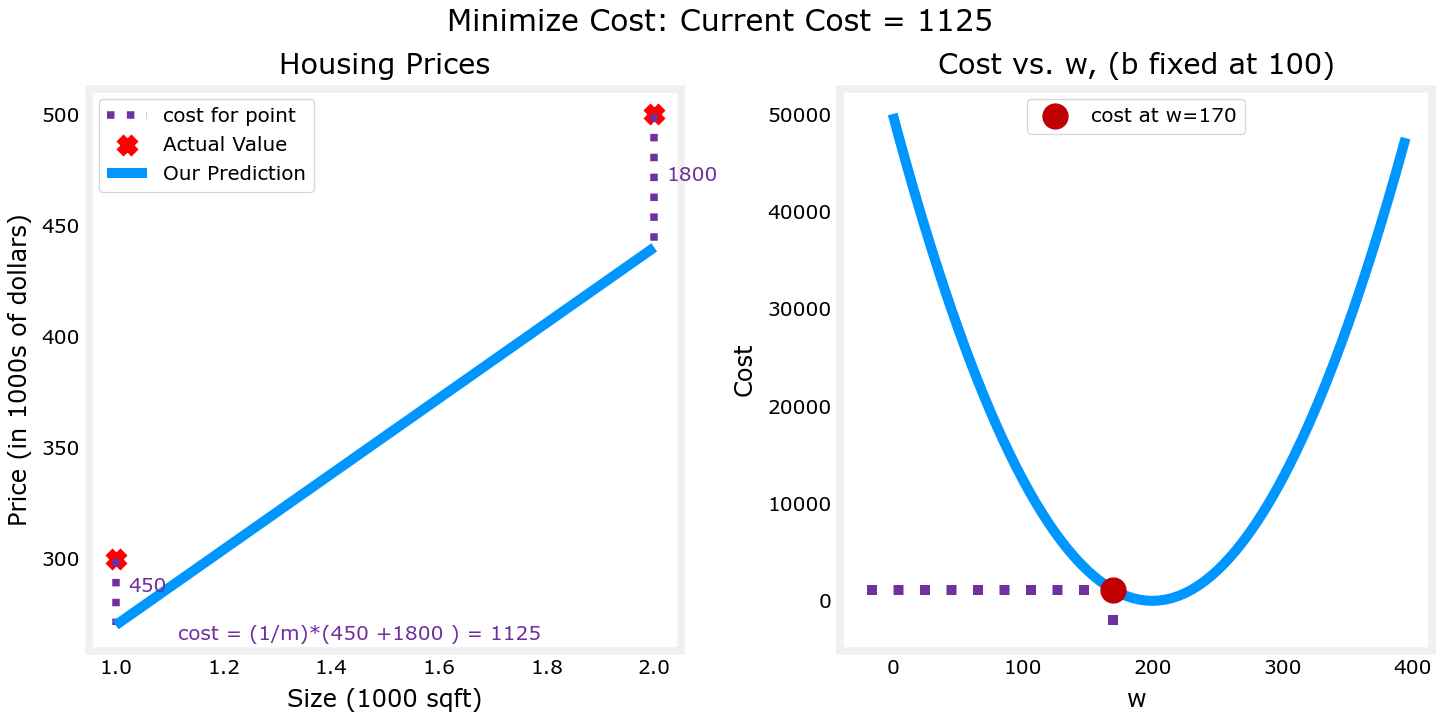
\includegraphics[width=\textwidth]{images/2.2_1}

\subsection*{$J(w, b)$ with two parameters $w$ and $b$}
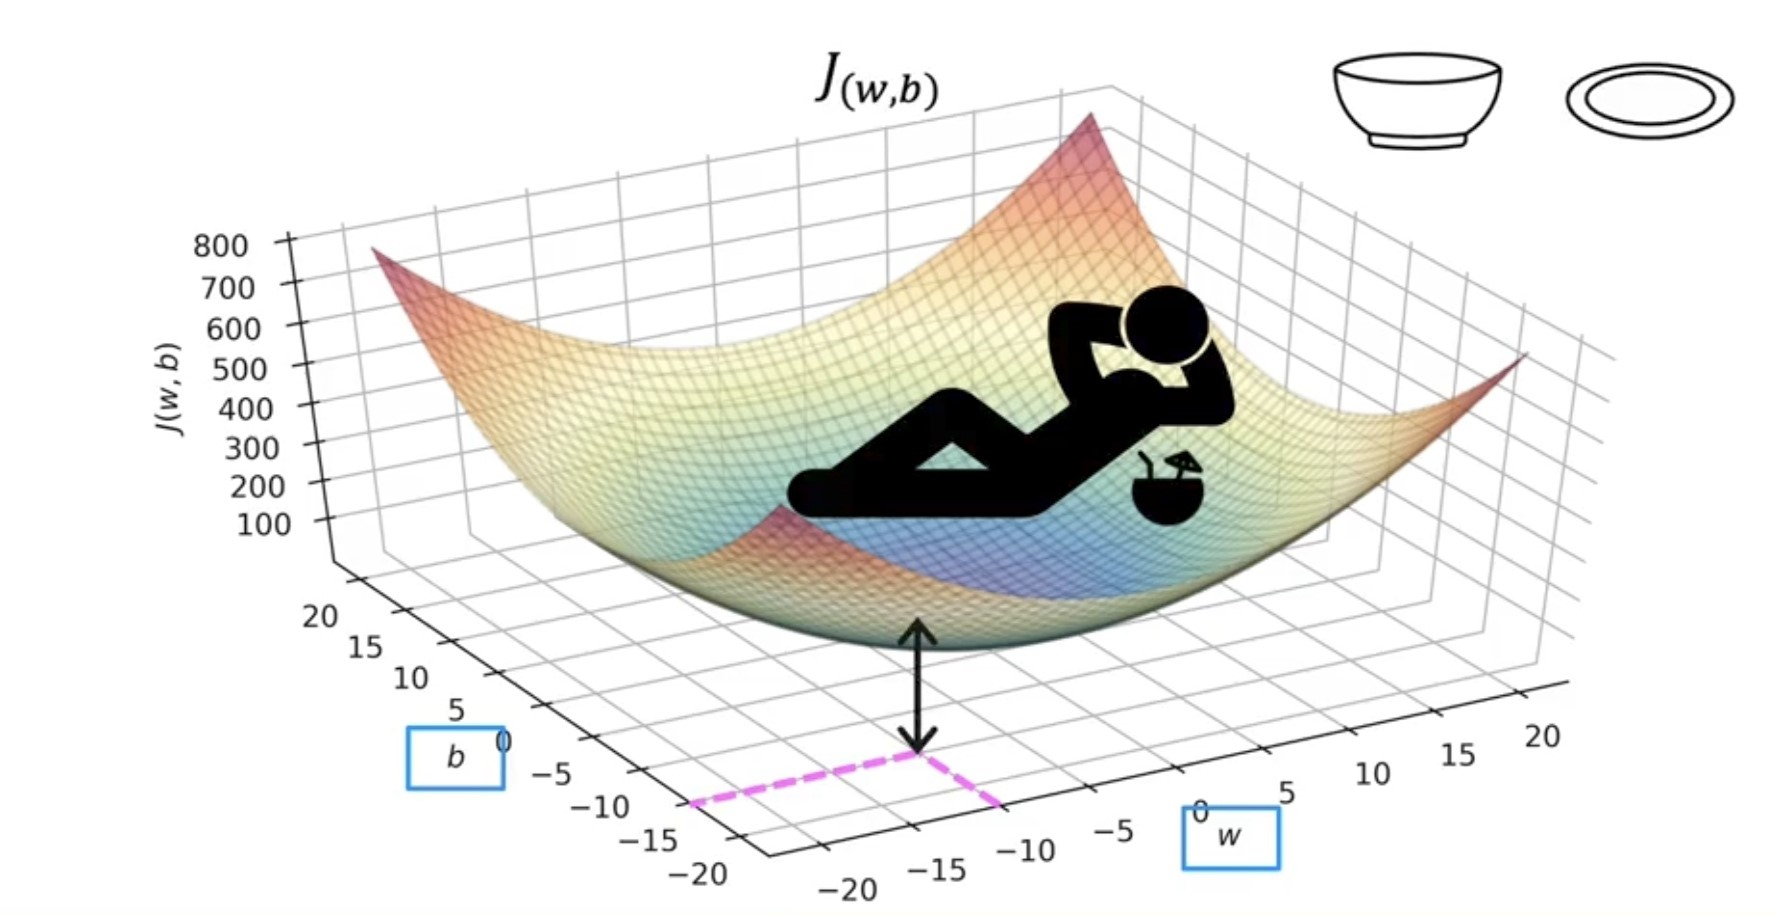
\includegraphics[width=\textwidth]{images/2.2_2}
\vspace{2em}
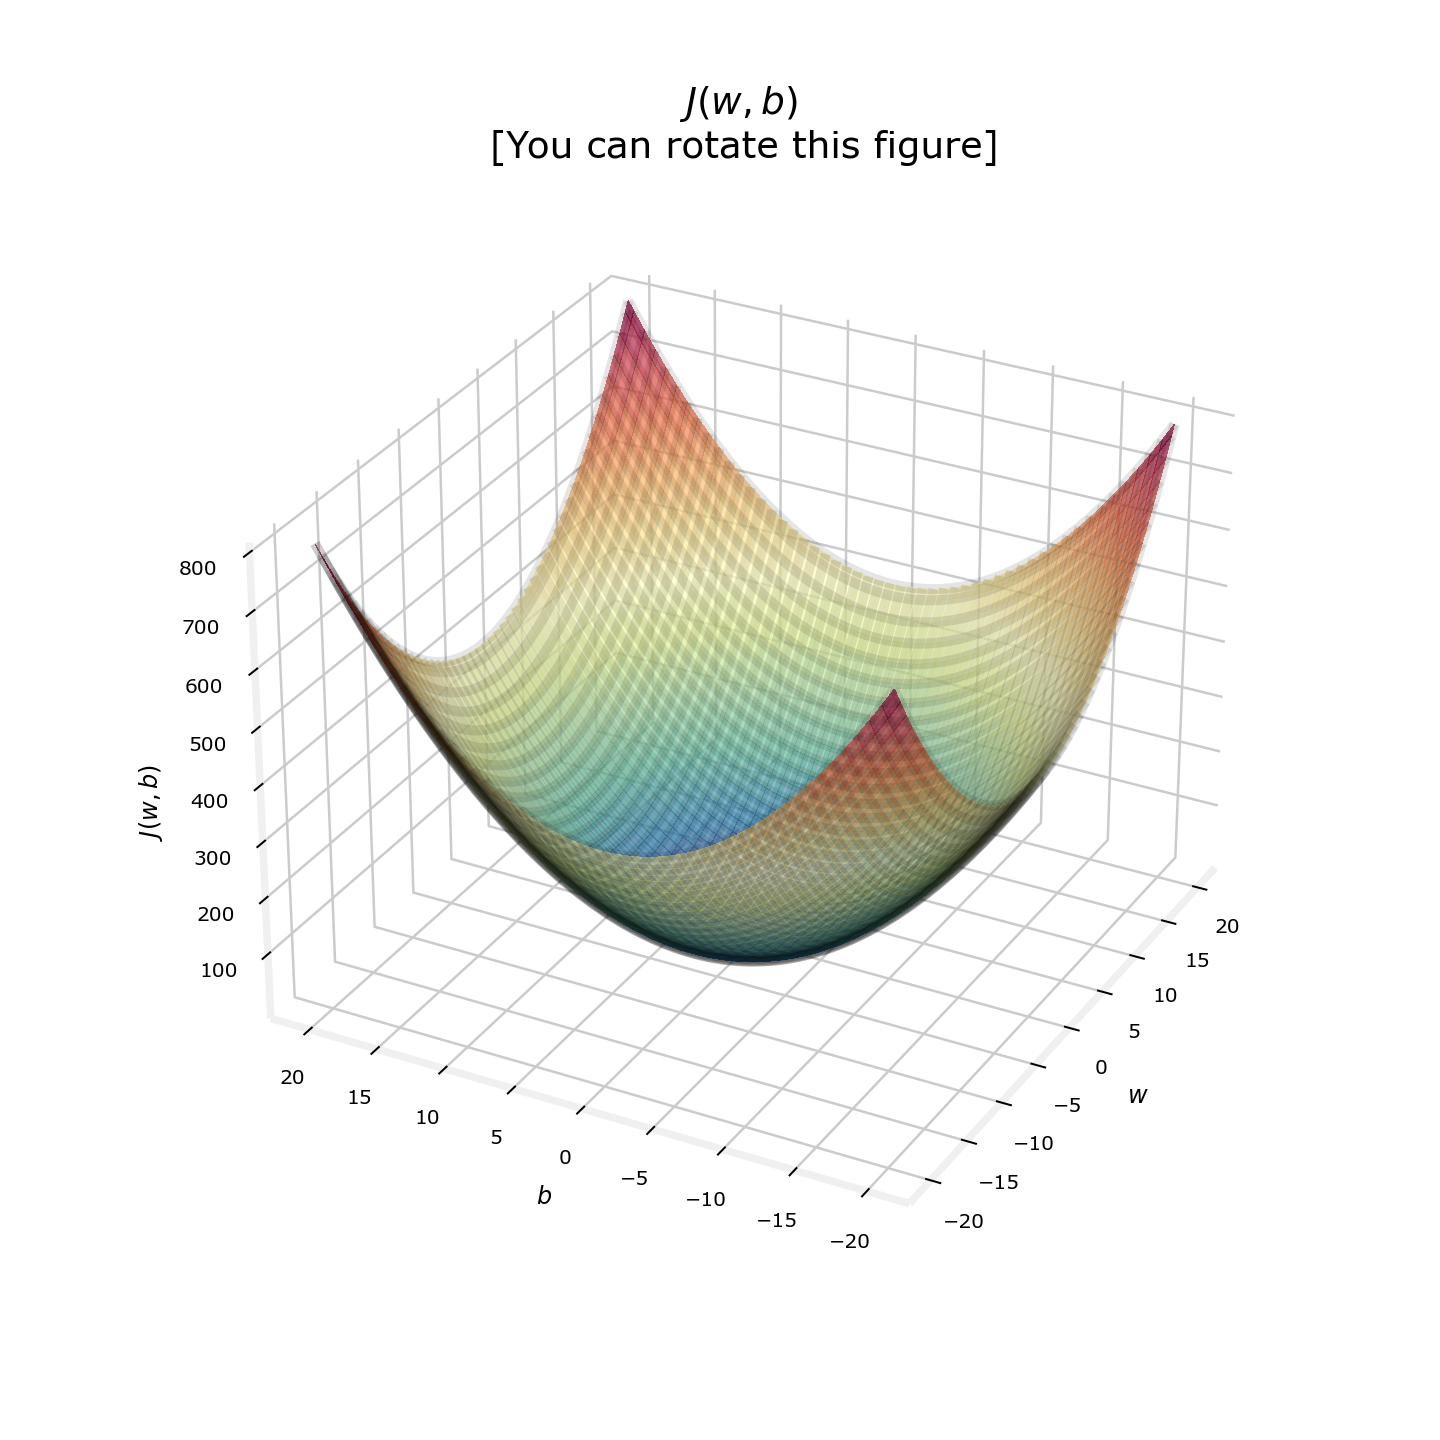
\includegraphics[width=\textwidth]{images/2.2_6}
\paragraph*{explaination}
The cost function $J(w, b)$ always has the shape of a ``soup bowl''.\par
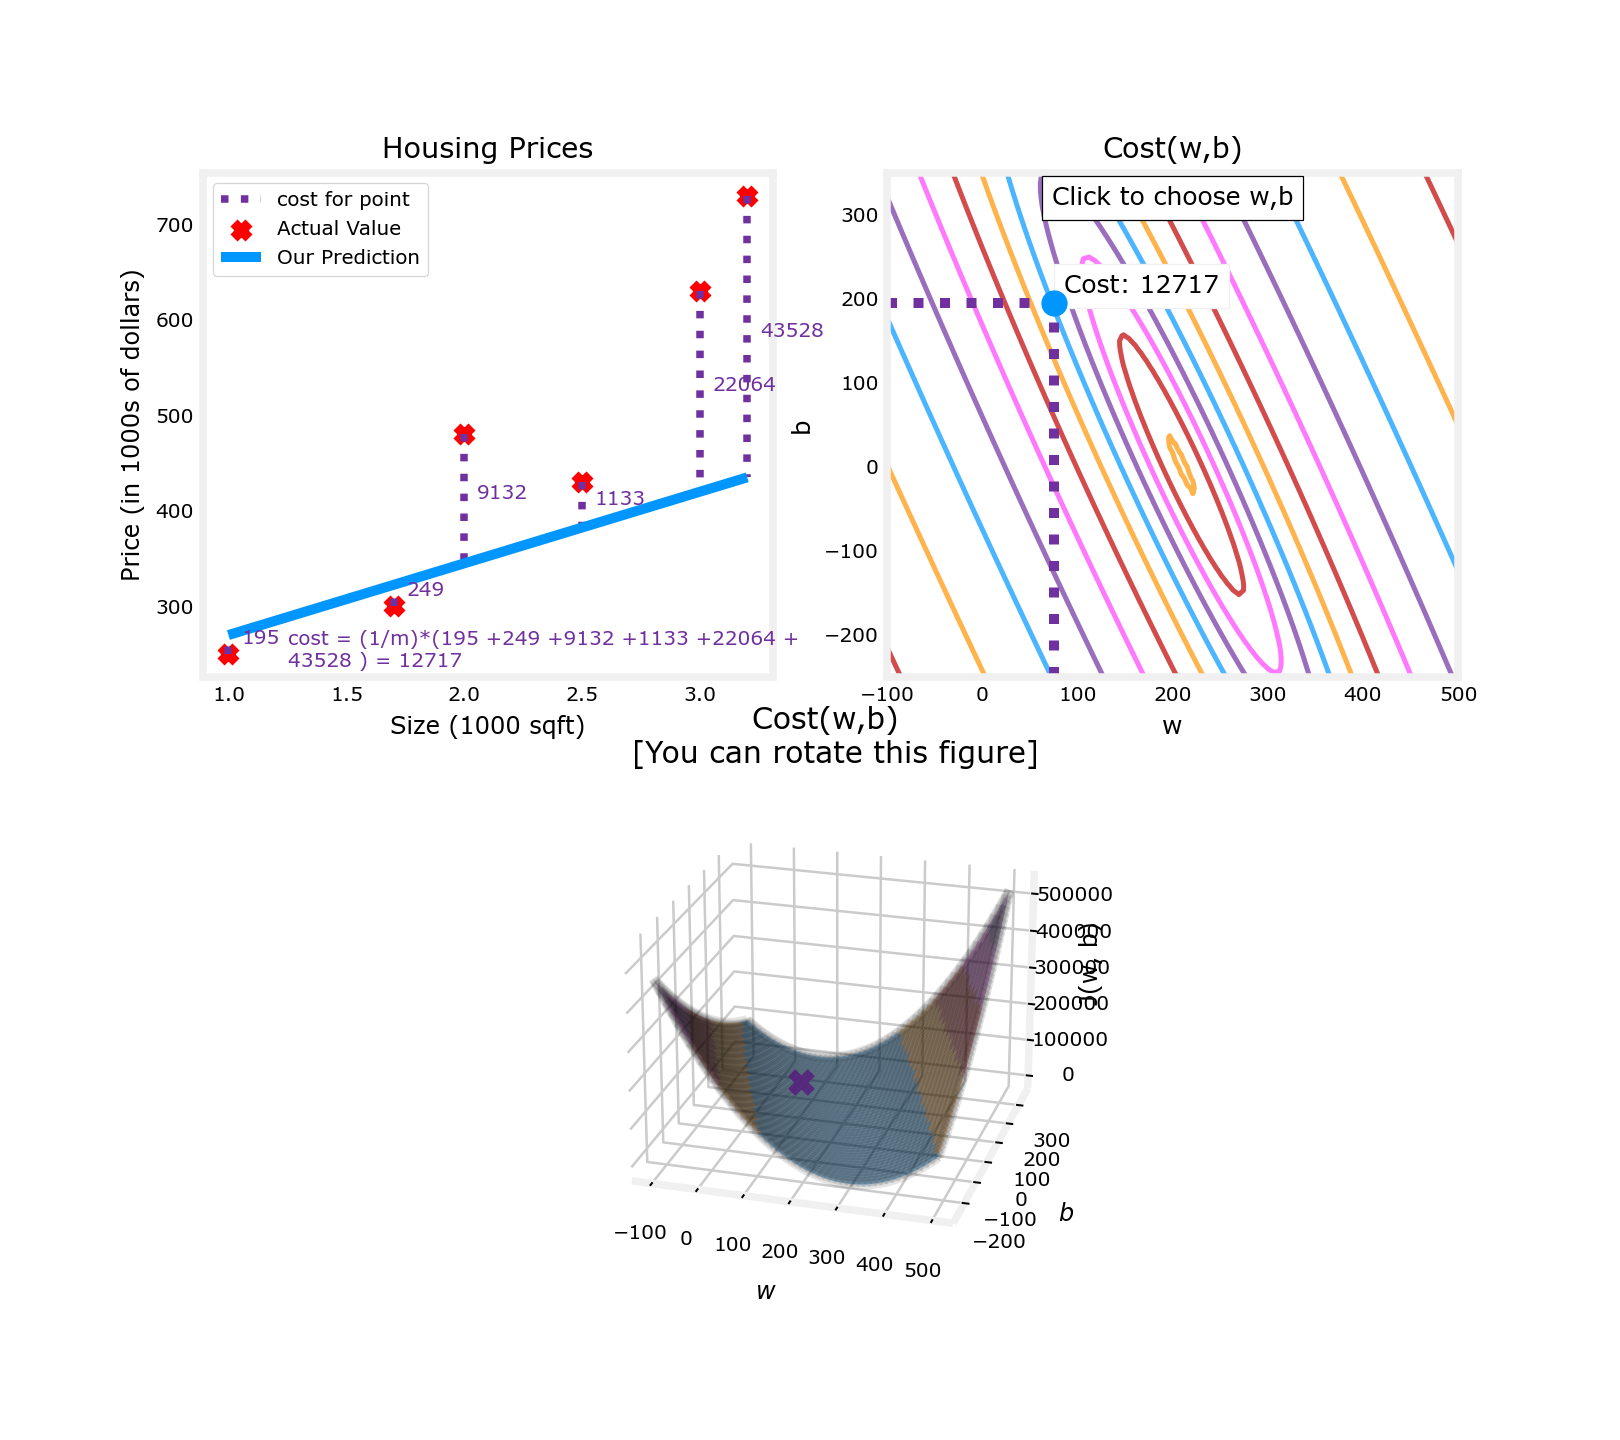
\includegraphics[height=0.7\textheight]{images/2.2_5}
\vspace{2em}
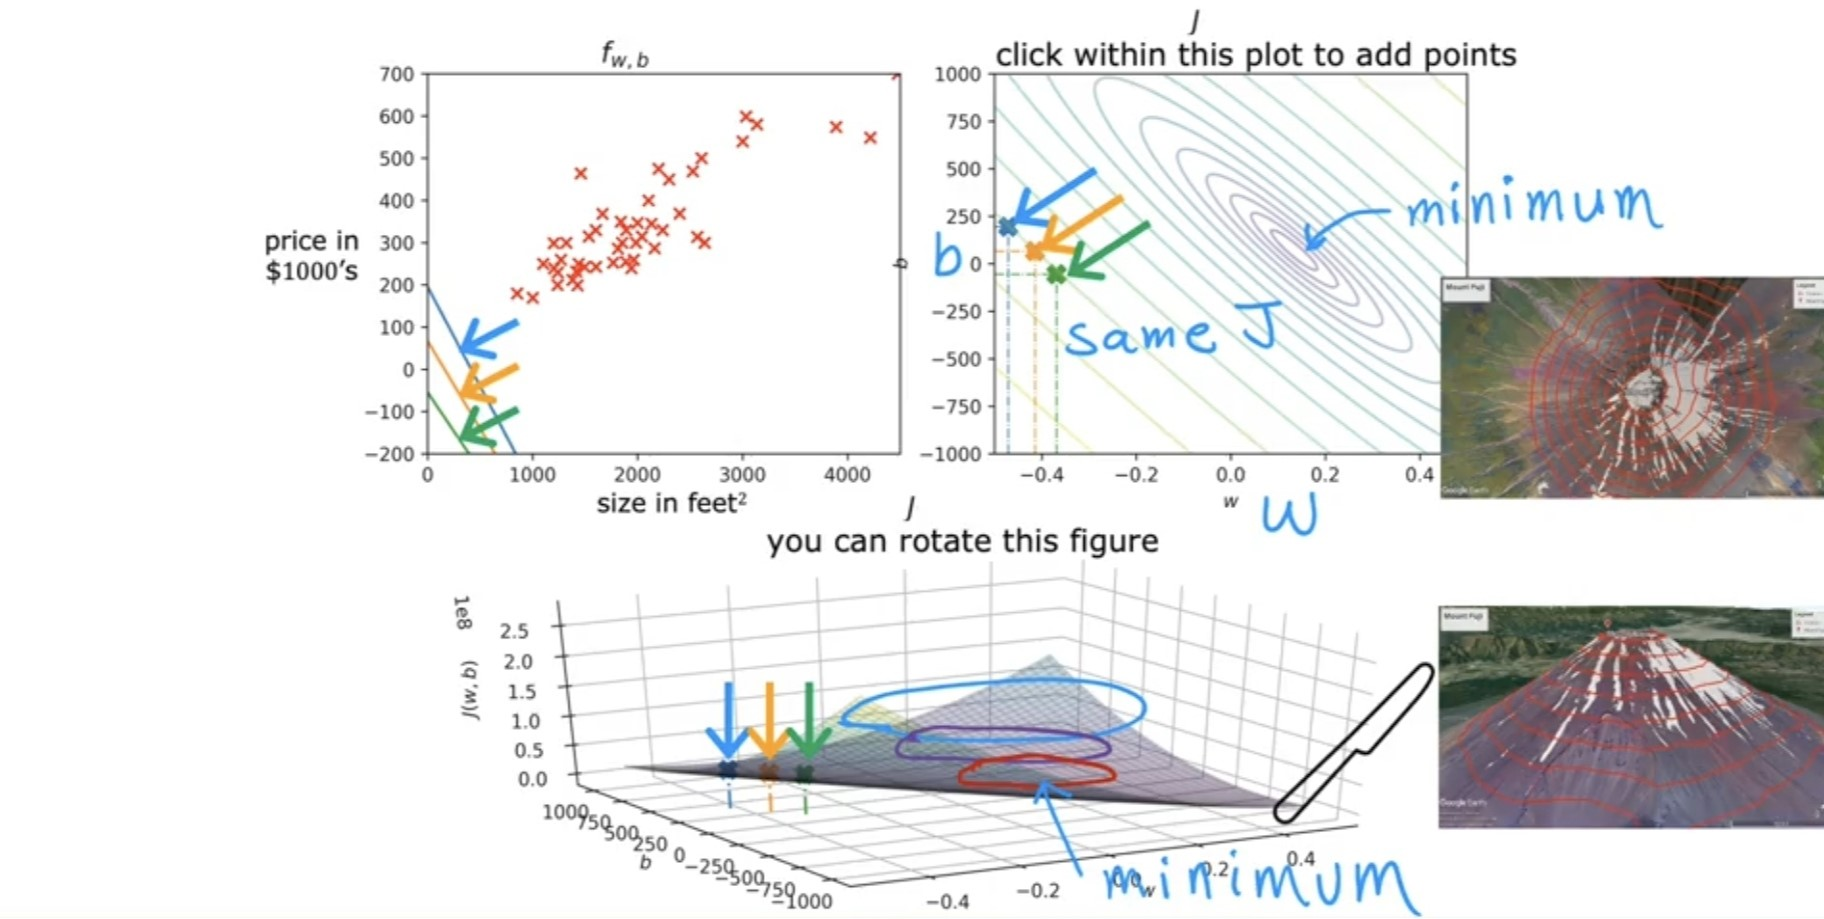
\includegraphics[width=\textwidth]{images/2.2_3}
\paragraph*{explaination}
The 3D plot can be transformed into a contour plot.\par